\documentclass[leqno]{article}
\usepackage{graphicx}
\usepackage[margin=1in]{geometry}
\usepackage{amsmath}
\usepackage{siunitx}
\usepackage{amsthm}
\usepackage{wrapfig}
\usepackage{subcaption}
\usepackage{amssymb}
\usepackage{booktabs}
\usepackage{multirow}
\usepackage[T1]{fontenc}
\usepackage[utf8]{inputenc}
\usepackage[italian]{babel}
\usepackage{stanli}

\usetikzlibrary{decorations.pathreplacing}
\usetikzlibrary{angles,quotes} 
\usetikzlibrary{circuits.logic.US,circuits.logic.IEC}

\begin{document}
	
	
	
	\title{Filtro doppio notch}
	\author{V. Brugnami 1027102, N. D'Agosta 1050342}
	\date{ 25 Maggio 2023}
	\maketitle
	
	\section{Abstract}
	Lo scopo di questo esperimento è quello di realizzare e studiare un filtro doppio-notch, ovvero un doppio circuito elimina banda, con l'obiettivo principale di misurare le due frequenze di notch e verificare la loro compatibilità con i valori teorici attesi. I risultati ottenuti sono riportati nella tabella seguente.
	
	\begin{table}[h]
		\begin{center}
			\begin{tabular}{ |c|c|c|c| } 
				\hline
				\textbf{Resistenza} & \textbf{Frequenze teoriche} & \textbf{Frequenze registrate} \\
				\hline
				\multirow{2}{6em}{$(680.0\pm0.4) \Omega$} & $1830Hz$ & $(1800\pm100) Hz$ \\ 
				\cline{2-3}
				& $10700Hz$ & $(10600\pm100)Hz$ \\ 
				\hline
				\multirow{2}{6em}{$(2194\pm1) \Omega$} & $1830Hz$ & $(1800\pm100)Hz$ \\ 
				\cline{2-3}
				& $10700Hz$ & $(10800\pm100)Hz$ \\ 
				\hline
				\multirow{2}{6em}{$(9974\pm5) \Omega$} & $1830Hz$ & $(1800\pm100)Hz$ \\ 
				\cline{2-3}
				& $10700Hz$ & $(10900\pm100)Hz$ \\ 
				\hline
			\end{tabular}
		\end{center}
		\caption{In tabella sono paragonati i valori delle frequenze teoriche e di quelle ottenute}
		\label{Tab intro}
	\end{table}
	
	Inoltre per studiare ulteriormente la funzione di risposta del circuito sono stati misurati sia il modulo che la fase e poi si è verificato che fossero compatibili con quelli teorici. Le risposta è stata positiva nel caso delle resistenze da $(2194\pm1) \Omega$ e di $(9974\pm5) \Omega$  con resistenze ricavate dal fit della fase di $(2181   \pm   19) \Omega$ e di $( 10345   \pm   90) \Omega$ ed una buona compatibilità tra la funzione teorica e i dati ricavati. Il circuito a $(680.0\pm0.4) \Omega$  non è risultato compatibile per la fase, il fit infatti da un risultato di $(648  \pm   7) \Omega$, e neanche per il modulo della funzione di risposta. 
	
	
	\section{Introduzione}
	Il "notch filter" doppio è un classico esempio di un filtro elimina banda, ovvero di un circuito in grado di non rispondere a determinate frequenze immesse. Il dispositivo è un circuito RLC composto da due gruppi di condensatore e induttore in parallelo, messi in serie con una resistenza. Sono i vari valori di capacità ($C_i$) e induttanze ($L_i$) che determinano le "frequenze di notch", ovvero le frequenze alle quali, se si misura la tensione ai capi della resistenza, questa risulta in linea teorica nulla. I due valori si ottengono da:
	\begin{equation}
		\nu_1 = \frac{1}{2\pi \sqrt{L_1 C_1}  } \; \; \;  
		\nu_2 = \frac{1}{2\pi \sqrt{L_2 C_2}  }
		\label{Freq. notch}
		\numberwithin{equation}{section}
	\end{equation}
	
	Si dimostra inoltre, utilizzando la tecnica dei fasori per l'analisi del circuito,
	che la tensione misurata ai capi della resistenza risulta sfasata rispetto a quella immessa nel circuito.
	Si riesce quindi a prevedere la funzione risposta
	\begin{equation}
		\label{Tensione uscente}
		V_{out} = V_{in} |H(\omega)| cos(\omega t + \phi(\omega)) 
	\end{equation}
	dove $H(\omega)$ rappresenta la funzione di risposta percentuale propria del circuito, e $\phi(\omega)$ lo sfasamento.
	Inoltre si possono poi ottenere anche informazioni riguardo alle buche della funzione considerando il fattore di qualità 
	\begin{equation}
		\label{qualità}
		Q = R\cdot \sqrt{\frac{C_i}{L_i}}
	\end{equation}
	Tanto più questo risulta alto, tanto più il circuito risulta sensibile solo alle frequenze di notch, ottenendo quindi come risposta una buca più stretta e di conseguenza meno profonda.
	Bisogna tenere presente però che questi valori teorici sono molto approssimati, in quanto nella realtà non si possono trascurare le resistenze propire delle induttanze e altri errori sistematici propri dell'apparato sperimentale. \'E necessario quindi analizzare il circuito tramite un modello teorico più preciso, studiato in Appendice (\ref{Modulo h} e \ref{fase})
	e capire se i valori ottenuti lo rispecchino. 
	In particolare, è necessario valutare se le frequenze di notch teoriche, ovvero le frequenze per le quali $H(\omega)$ è minima, sono compatibili con quelle misurate.
	
	
	
	
	
	
	\section{Apparato sperimentale e svolgimento}
	
	\usetikzlibrary {circuits.ee.IEC}
	\begin{figure}[h]
		\begin{center}
			\begin{tikzpicture}[circuit ee IEC,x=3cm,y=2cm,semithick,
				every info/.style={font=\footnotesize},
				small circuit symbols,
				set resistor graphic=var resistor IEC graphic,
				set diode graphic=var diode IEC graphic,
				set make contact graphic= var make contact IEC graphic]
				\label{circuito}
				% Let us start with some contacts:
				\point{a}{0.}{0.};
				\point{b}{0.}{1.6};
				\point{c}{0.4}{1.6};
				\point{d}{0.4}{1.2};
				\point{e}{0.4}{2.};
				\point{f}{1.2}{1.2};
				\point{g}{1.2}{2.};
				\point{h}{1.2}{1.6};
				\point{i}{1.6}{1.6};
				\point{l}{1.6}{0.0};
				\point{m}{1.2}{0.0};
				\point{n}{1.2}{-0.4};
				\point{o}{1.2}{0.4};
				\point{p}{0.4}{0.4};
				\point{q}{0.4}{-0.4};
				\point{r}{0.4}{0.0};
				\point{s}{0.8}{2.};
				\point{t}{0.8}{0.4};
				
				\draw (b)--(c)--(e);
				\draw (c)--(d);
				\draw (g)--(f);
				\draw (h)--(i);
				\draw (i) to  [resistor={info ={$R$}}]  (l);
				\draw (l)--(m);
				\draw (n)--(o);
				\draw (a) to [battery] (b);
				\draw (d) to [capacitor={info = {$C_1$}}] (f);
				\draw (n) to [capacitor={info = {$C_2$}}] (q);
				\draw (e) to [inductor = {info = {$L_1$}}] (s);
				\draw (s) to [resistor={info ={$R_1$}}] (g);
				\draw (p) to [inductor= {info ={$L_2$}}] (t);
				\draw (t) to [resistor={info ={$R_2$}}] (o);
				\draw (a)--(r);
				\draw (p)--(q);
				
			\end{tikzpicture}
		\end{center}
		\caption{Schema del circuito realizzato}
		\label{circuito}
	\end{figure}
	
	Per la realizzazione del circuito è stata utilizzata la breadbord della scheda NI ELVIS II. Come raffigurato dallo schema in Fig. \ref{circuito}
	il filtro doppio notch è costituito da due maglie composte da un condensatore in parallelo con un'induttore, messe in serie ad una resistenza.
	Per misurare i vari valori delle componenti del circuito, sono state usate le strumentazioni del multimetro digitale della ELVIS, ed in particolare per la resistenza è stato usato un tester digitale, ottenendo dei valori di:
	
	\begin{itemize}
		\item $L_1 = 47.9 \pm 0.5 mH$
		\item $R_1 = 128.1\pm 0.2\Omega$
		\item $C_1 = 0.158 \pm 0.002 \mu F$
		\item $L_2 = 0.479 \pm 0.005 mH$
		\item $R_2 = 2.252 \pm 0.004 \Omega$
		\item $C_2 = 0.466 \pm 0.005 \mu F$
	\end{itemize}
	
	
	Per il calcolo degli errori sui dati misurati sono state consultate le specifiche della ELVIS.
	Il tutto è sottoposto a una tensione generata dalla funzionalità "function generator" dalla ELVIS variabile nel tempo. In particolare, va considerata la resistenza interna della scheda, che è dichiarata essere di $R_{fgen} = 50 \Omega$.
	
	
	Poichè l'obiettivo risulta essere quello di misurare l'ampiezza della tensione ai capi della resistenza, è stato necessario per prima cosa calcolare l'incertezza statistica sul voltaggio. Per fare ciò è stato costruito un semplice circuito formato dalla sola resistenza nel quale è stata immessa un'onda quadra di lungo periodo. In questo modo è stato possibile acquisire un campione statistico di dati distribuito attorno al valore di input, per riuscire quindi ad ottenere la deviazione standard della distribuzione ottenuta e quindi l'errore da associare alle successive misure della tensione. 
	
	\begin{wrapfigure}{r}{0.65\textwidth} 
		\centering
		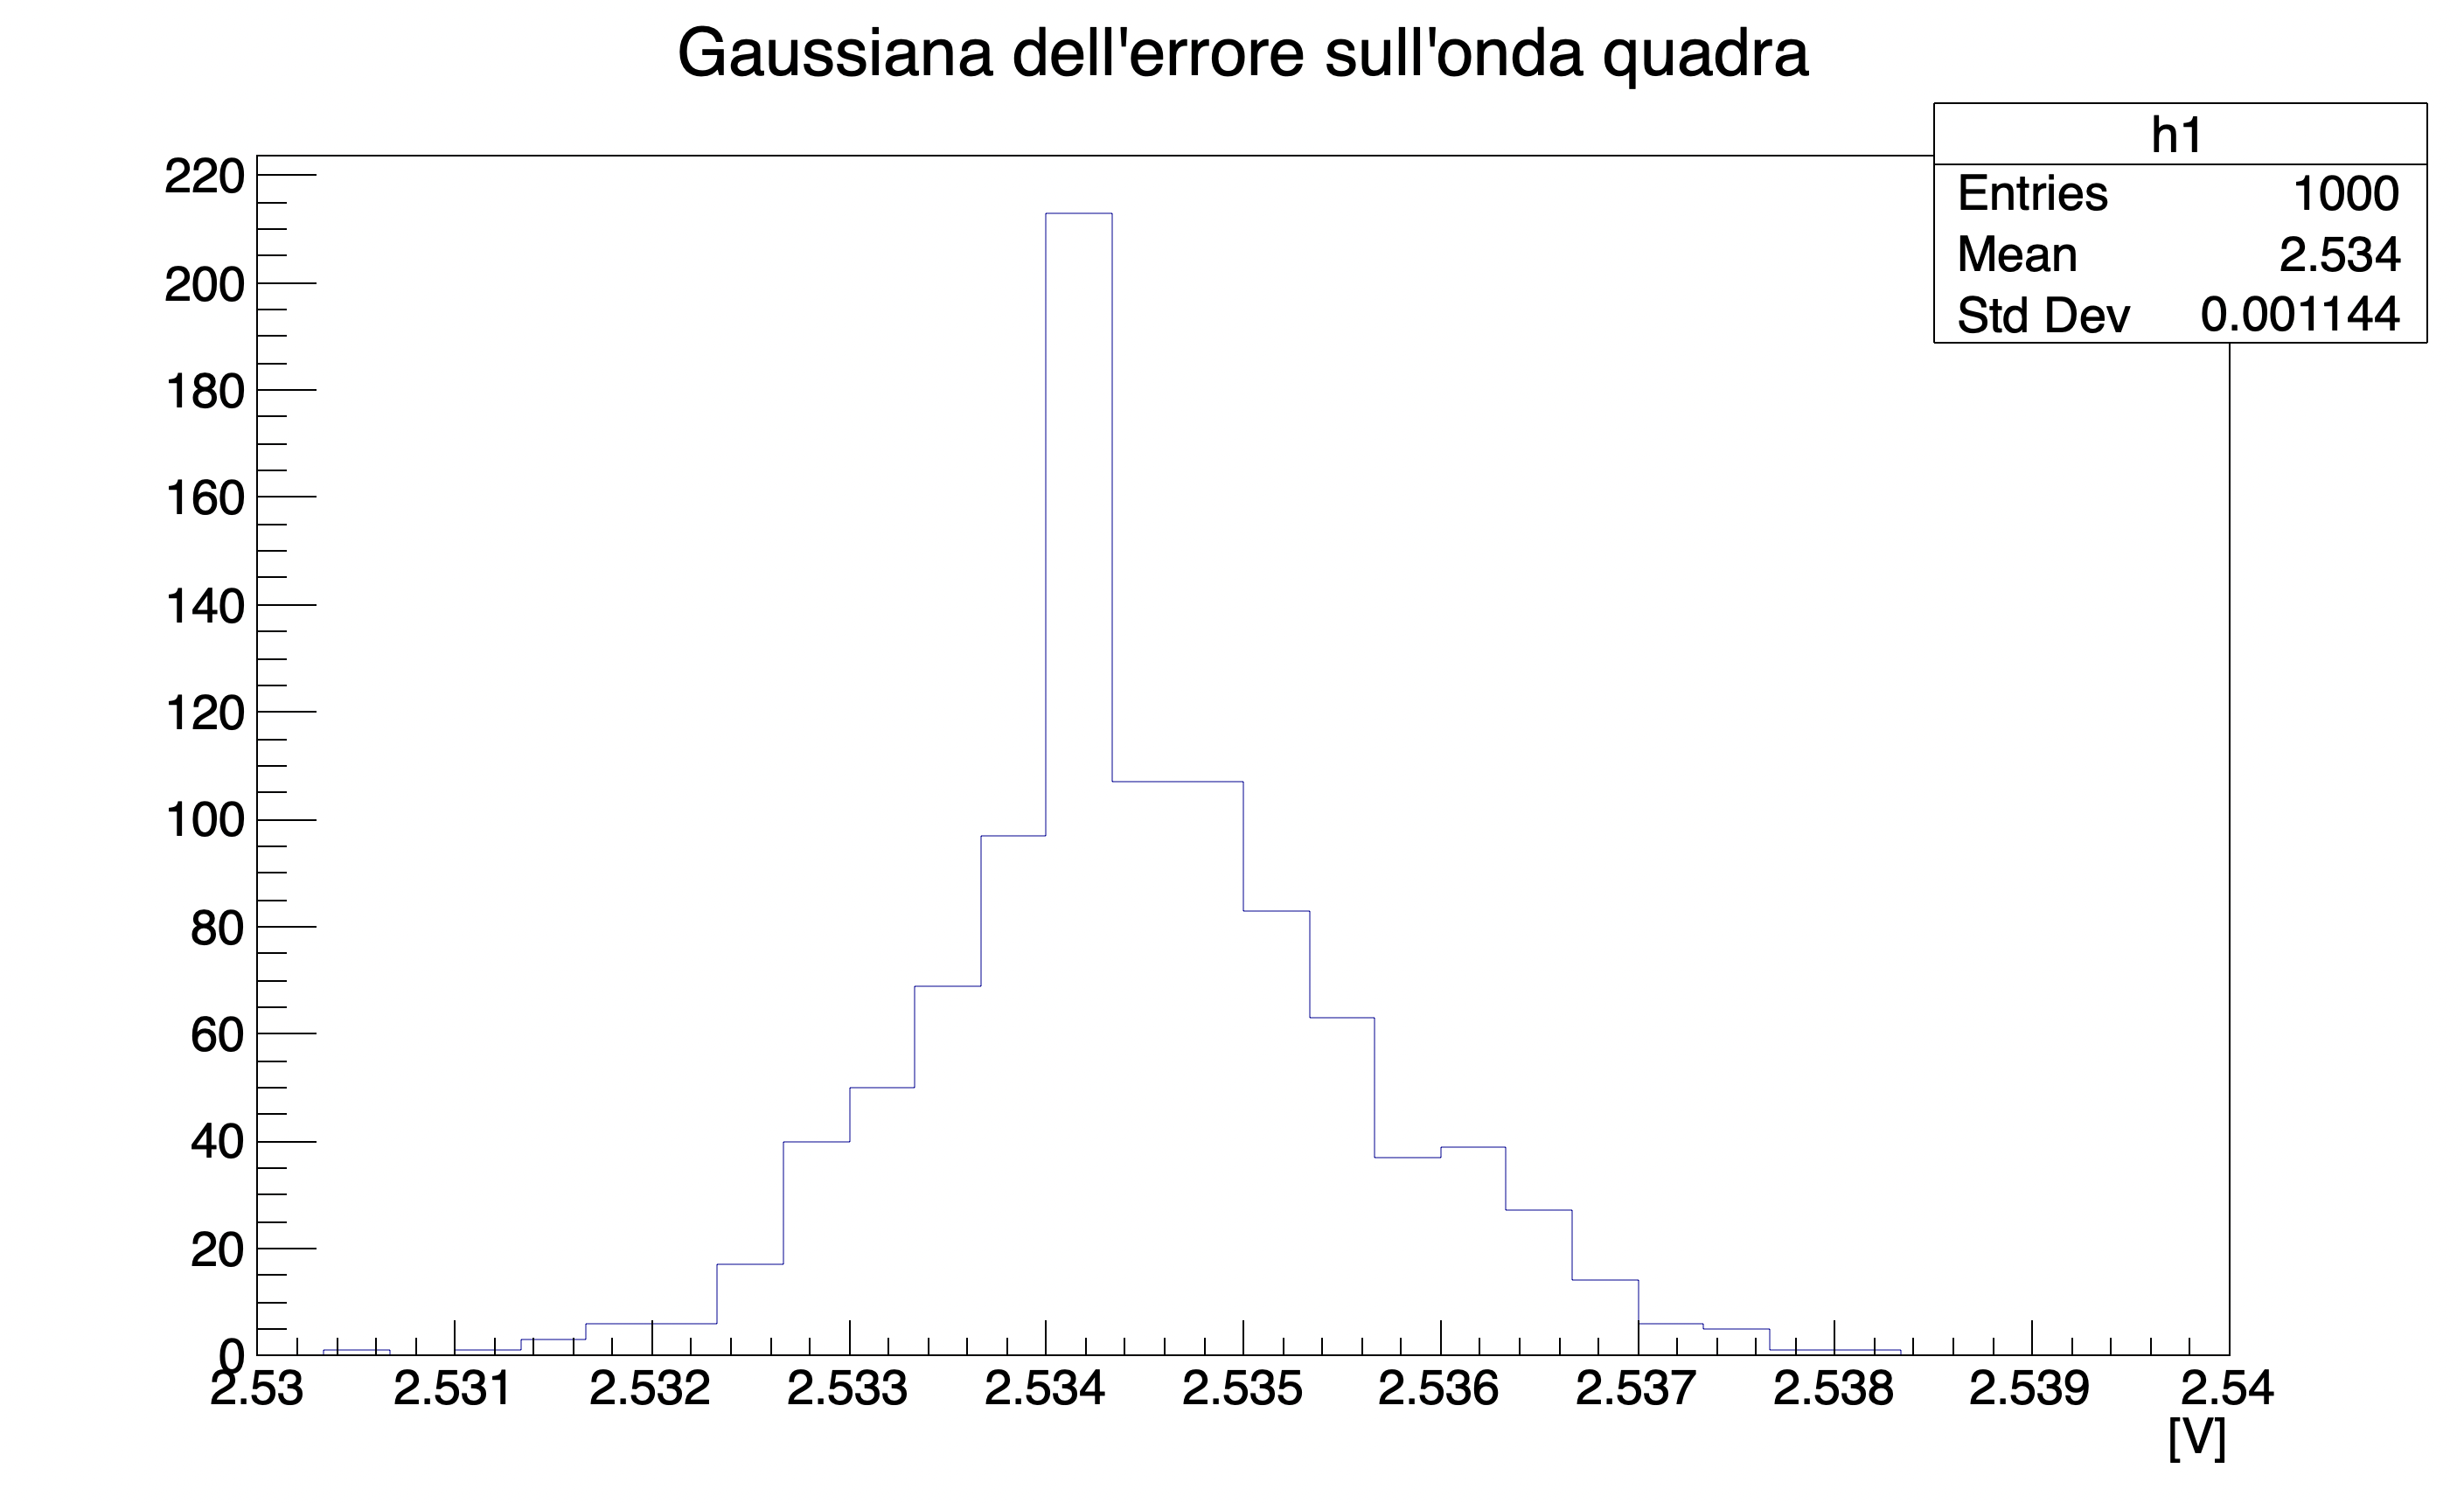
\includegraphics[scale=0.25]{Errore.png}
		\caption{"Distribuzione dei voltaggi per l'onda quadra"}
		\label{errore}
	\end{wrapfigure}
	
	Successivamnte è stato immesso nel circuito un voltaggio di 5V di frequenza crescente tra 300 Hz e 15000 Hz, con passi di 100 Hz,
	e sono poi state prese le misure della risposta ai capi della resistenza utilizzando tre valori di R diversi, pari a $(680.0\pm0.4) \Omega$, $(2194\pm1)  \Omega$, $(9974\pm5) \Omega$.
	Il range della frequenza è stato scelto in quanto si attendono, in base alle relazioni (2.1), due valori per le frequenze di notch pari a 
	1830 Hz e 10700 Hz.
	Contemporaneamente, è stato anche generato un grafico rappresentante la fase della tensione in funzione della frequenza, così da ottenere tutti i dati per verificare la compatibilità della \eqref{Tensione uscente} teorica con quella sperimentale. Anche in questo caso è servita una seconda misura per riuscire a determinare l'errore sistematico della ELVIS nella presa dati della fase.
	La ELVIS infatti acquisice dati con un certo intervallo temporale , il che porta alla misura di uno sfasamento in realtà non effettivamente presente dovuto al fatto che ad alte frequenze questa distanza temporale di acquisizione diventa rilevante. Immetendo una tensione di frequenza variabile, è stata quindi analizzata la fase ai capi del generatore per trovare l'errore in funzione della frequenza, senza il quale la fase dovrebbe essere nulla.
	
	
	
	
	
	
	\section{Risultati e discussione}
	Lo studio dei risultati ottenuti si può riassumere nell'analisi del modulo e della fase della funzione di risposta $H(\omega)$, con particolare attenzione alle frequenze di notch.
	\subsection{Analisi del modulo e delle frequenze di notch}
	
	\begin{figure} [h!]
		\centering
		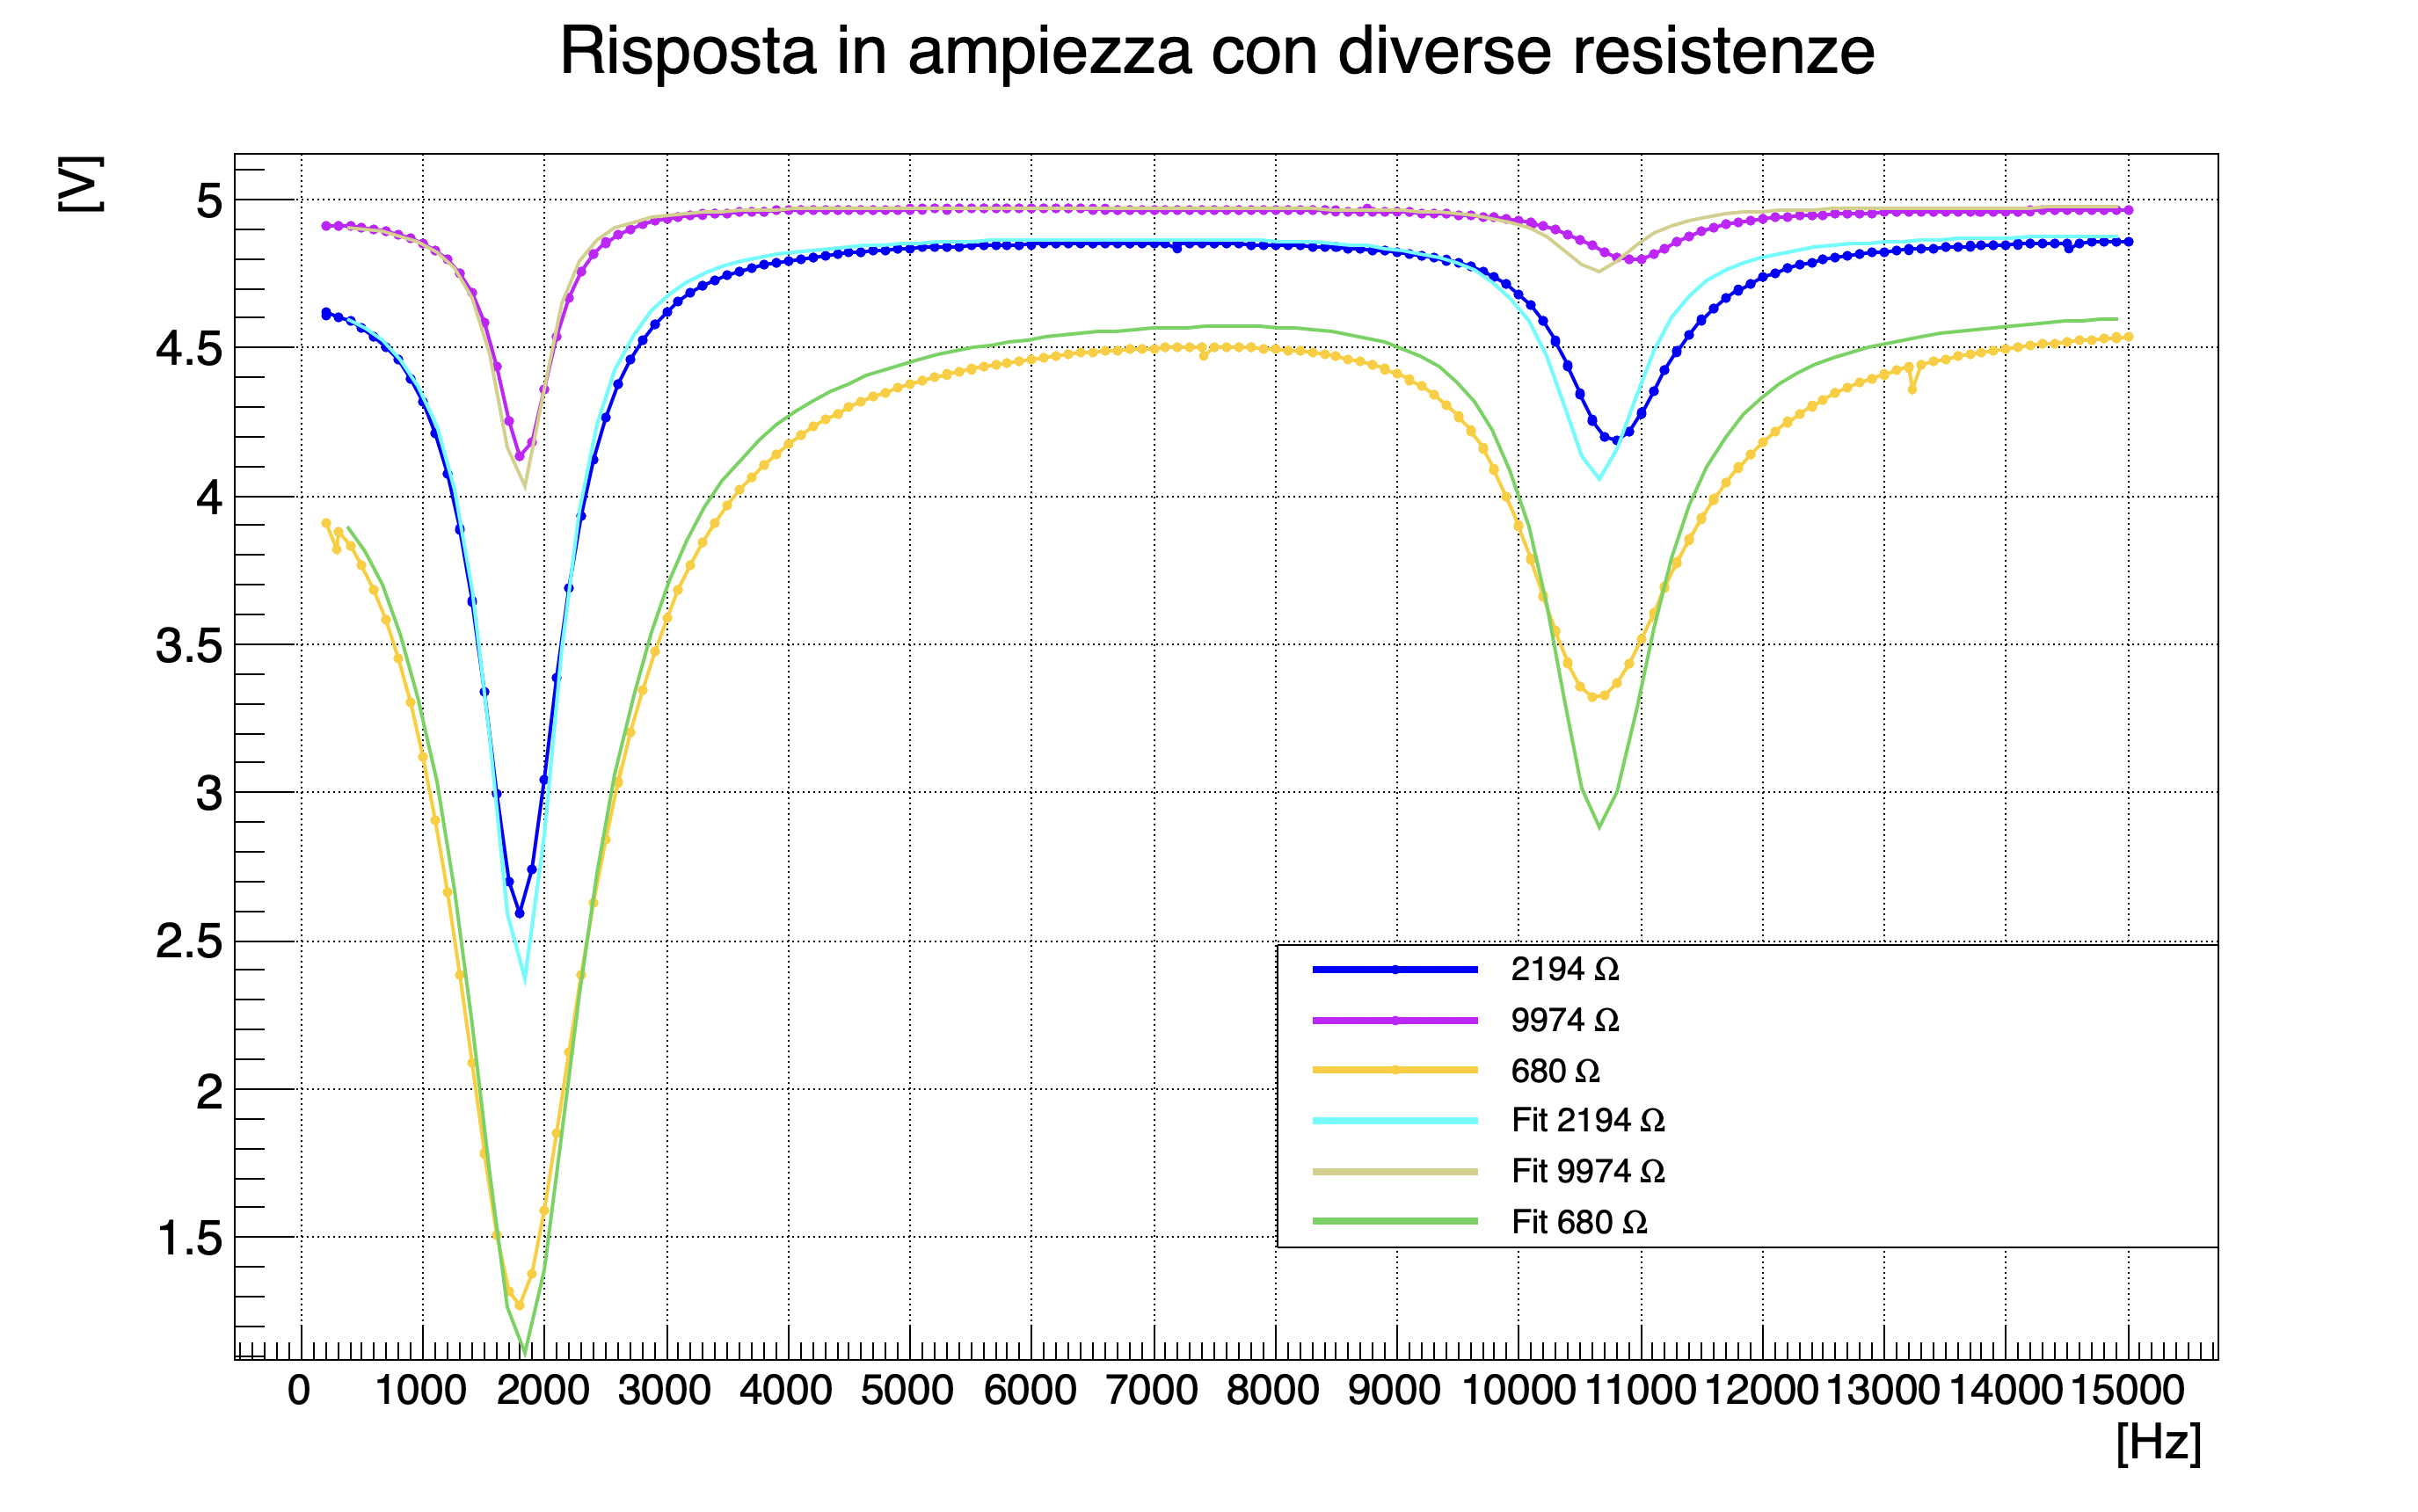
\includegraphics [scale=0.23] {Rispostampiezza.png}
		\caption{Riportati i dati acquisiti per le tre resistenze e i rispettivi fit con la funzione teorica}
		\label{RisAmp}
	\end{figure}
	
	In Fig. \ref{RisAmp} si vede l'andamento della tensione ai capi della resistenza in funzione della frequenza. Qualitativamente si capisce subito che il circuito si comporta come previsto dalla teoria, con buche a frequenze simili a quelle calcolate precedentemente. Si sono poi calcolati i due fattori di qualità propri del circuito secondo la \ref{qualità}, ottenendo  e $Q_1 = R\cdot 1.8 \cdot 10^{-3}$ e $Q_2 = R\cdot 3.1 \cdot 10^{-2}$, dove è stato lasciato il parametro R in quanto ininfluente per paragonare i due valori.
	Come previsto dei due quello associato alla buca più stretta e meno profonda rosulta essere proprio $Q_2$, il maggiore dei due.
	
	Per capire però se effettivamente il comportamento è compatibile con quello atteso, è necessario uno studio quantitativo dei dati del fit.
	Per prima cosa sono state calcolare le incertezze da associare ai vari valori.
	Come errore sulle frequenze si è preso l'intervallo dei passi con cui durante l'acquisizione la frequenza immessa aumentava, che come visto precedentemente risulta essere di 100 Hz.
	Per quanto riguarda l'ampiezza invece, come già spiegato, si deve considerare 3 volte la deviazione standard della gaussiana in Figura \ref{errore} che risulta pari a $(0.004)V$.
	
	In virtù di ciò è stato possibile analizzare la compatibilità dei valori attesi con quelli ottenuti.
	Analizzando il caso con R= 680 $\Omega$, la funzione teorica in \eqref{Modulo h} ammette due minimi, precisamente a 1820 Hz e 10665 Hz, e i corrispettivi voltaggi pari a 1.095 V e 2.97 V. Ciò che si ottiene dai dati sperimentali invece sono due valori per le frequenze di notch di $(1800 \pm 100)Hz$ e $(10600 \pm 100)Hz$, e per le ampiezze di $( 1.269 \pm 0.004)V $ e $ (3.322 \pm 0.004)V$ quindi non risultano compatibili le ampiezze e una delle due frequenze di notch.
	%Che dici cosi?
	Il problema potrebbe essere attribuito al fatto che delle tre resistenze di carico questa è la inferiore, e risultano quindi incisive le approssimazioni utilizzate.
	
	
	
	Analizzando i casi delle resistenze da $2194\Omega$ e $9974\Omega$ è stata riscontrata invece una maggiore compatibilità sia per le frequenze di notch con dei valori rispettivamente di $(1800 \pm 100)Hz$, $(10800 \pm 100)Hz$ e di $(1800 \pm 100)Hz$ e $(10900 \pm 100)Hz$ che nell'ampiezza delle frequenze di $( 2.593 \pm 0.004)V $ , $( 4.185 \pm 0.004)V $ e di $ (4.132 \pm 0.004)V $, $ (4.795 \pm 0.004)V $ che risultano discretamente compatibili considerando quelli teorici di $2.385V, \;   4.135V$ e di $ 4.03V , \;  4.78V$ tenendo anche conto del fatto che l'ampiezza misurata non è esattamente alla frenquenza di notch a causa dei salti da 100Hz. Il che dimostra una buona compatibilità tra il modello teorico e i risultati sperimentali quando le altre resistenze del circuito risultano meno incidenti.
	
	\subsection{Analisi della fase}
	\begin{figure} [h!]
		\centering
		\includegraphics [scale=0.25] {fase.png}
		\caption{Dati ottenuti dello sfasamento (in gradi) in funzione della frequenza}
		\label{Fase}
	\end{figure}
	Dalla Fig. \ref{Fase} si vede che anche per la fase i dati acquisiti sembrano adattarsi bene al modello teorico con cui si è ottenuto il fit. Si nota infatti come le inversioni della fase avvengono propio alle frequenze di notch.
	In particolare se si studiano i punti di flesso della funzione \eqref{Faseeq} si ottiene un nuovo metodo per il calcolo delle frequenze critiche. Si noti che i valori teorici sono esattamente gli stessi ottenuti dallo studio dei minimi della funzione $|H(\omega)|$. Anche i risultati del fit, eseguito sulla resistenza di carico lasciando gli altri sei parametri parametri fissati, sono risultati positivi nel caso delle resistenze da $2194\Omega$ e $9974\Omega$ ottenendo dei valori di $(2181   \pm   19) \Omega$ e di $( 10345   \pm   90) \Omega$ e non compatibili nel caso della resistenza da $680\Omega$ riportando un valore di fit di $(648  \pm   7) \Omega$.
	
	\section{Conclusioni}
	In conclusione si può affermare con sufficiente certezza che il circuito studiato si è comportato seguendo il modello teorico previsto in precedenza. Le frequenze ottenute sono infatti risultate compatibili con le frequenze attese, e lo stesso per i valori dei rispettivi voltaggi. 
	Anche lo studio dei fattori di qualità ha portato ai risultati sperati, in quanto le buche sono risultate tanto più strette tanto più alto risulta essere Q. Poichè infatti esso dipende linearmente dalla resistenza del circuito, dal grafico si nota come con le resistenze maggiori la buca risulta essere meno profonda e meno larga.
	Pertanto anche i fit, sia della risposta che della fase, sono risultati ottimali.
	L'unico risultato negativo è stato ottenuto per la resistenza di $680 \Omega$, ottenendo dal fit un valore di $(648 \pm 7) \Omega$, probabilmente in quanto, essendo la resistenza inferiore delle tre, le piccole resistenze trascurate del circuito sono risultate influenti.
	
	\setcounter{section}{0}
	\renewcommand{\thesection}{\Alph{section}}
	\section{Appendice}
	\subsection{Analisi del circuito}
	
	
	Calcolo di $\mathbb{H}( \omega)$:
	
	\begin{equation}
		\dfrac{1}{\mathbb{Z}_I}= \dfrac{1}{R_1+i\omega L_1} + i \omega C_1 = \dfrac{1 + i \omega C_1 (R_1 + i \omega L_1)}{R_1 + i \omega L_1}
		\label{Zi}
	\end{equation}
	
	Da cui : 
	\begin{equation}
		\mathbb{Z}_{eq} = \dfrac{R_1 + i \omega L_1}{1 + i \omega C_1 (R_1 + i \omega L_1)} + R + \dfrac{R_2 + i \omega L_2}{1 + i \omega C_2 (R_2 + i \omega L_2)} 
		\label{Zeq}
	\end{equation}
	\subsection{$|\mathbb{H}(\omega)|$ }
	
	Riprendendo la \eqref{Zi} e la \eqref{Zeq}, definendo infine: 
	
	
	\begin{itemize}
		\item $A =  1- \omega^2 C_1 L_1 $
		\item $B = \omega C_1 R_1 $
		\item $C = 1- \omega^2 C_2 L_2$
		\item $D = \omega C_2 R_2$
		\item $E = R_1 C - \omega L_1 D +(R+R_{fgen})AC - (R+R_{fgen})BD + R_2A - \omega L_2 B$
		\item $F = \omega L_1 C + R_1 D + (R+R_{fgen})BC + (R+R_{fgen})DA + \omega L_2 A + B R_2$
	\end{itemize}
	Otteniamo un valore di $H $ : 
	
	\begin{equation}
		\begin{aligned}
			\mathbb{H} & = \dfrac{R(A+ i B)(C+iD)(E-iF)}{(E + iF)(E - iF)} = \\
			& =\dfrac{R }{E^2 + F^2} \left( (ACE - BDE + BCF + FDA) + i ( BFD - ACF + BCE +DAF )\right)
		\end{aligned}
	\end{equation}
	\vspace{0.5cm}
	
	\begin{equation}
		\label{Modulo h}
		\begin{aligned}
			|\mathbb{H}| &= \dfrac{R}{E^2+ F^2}\sqrt{(ACE-BDF+BCF+FDA)^2+ (BDF-ACF+BCE+DAE)^2} = \\
			&= R\sqrt{\dfrac{(AC-BD)^2 + (BC+DA)^2}{E^2 + F^2 }}  
		\end{aligned}
	\end{equation}
	
	
	\subsection{$\mathbb{\phi(\omega)}$}
	Per l'analisi della fase, è sufficiente utilizzare la relazione dei numeri complessi
	\begin{equation}
		\label{fase}
		\phi = arctg(\frac{Imm{H}}{Re{H}})
	\end{equation}
	Si ottiene, sempre in riferimento alle definizioni del paragrafo precedente,
	\begin{equation}
		\phi = arctg(\frac{F(BD-AC)+E(BC+DA)}{F(BC+FD)+E(AC-BD)})
		\label{Faseeq}
	\end{equation}
	
\end{document}